\documentclass[12pt]{comjnl}

\usepackage{amsmath}

%\copyrightyear{2009} \vol{00} \issue{0} \DOI{000}
\linespread{1.5}

\begin{document}

\title[Hashtag Segmentation of Conversational Tweets in Turkish]{Hashtag Segmentation of Conversational Tweets in Turkish, Modelling Segmentation Approach Final Report}
\author{Utku Saridede, Sevket Topuz\\
Advisor: Ass. Prof. Arzucan Ozgur\\
Co-Advisor: Arda Çelebi}
\affiliation{Degree of Bachelor of Science \\
Natural Language Processing and Informational Retrival, Department of
Computer Engineering, Bogazici University, Istanbul
Bebek 34342, TR} \email{utku.saridede@boun.edu.tr, sevket.topuz@boun.edu.tr}

\shortauthors{Hashtag Segmentation of Conversational Tweets in Turkish}

\received{07 October 2015}
\revised{12 January 2016}

\keywords{Twitter; Tweet; Tweets; Hashtag; Segmentation; Turkish; Conversational Tweets;
		Hashtag Segmentation}

\begin{abstract}	
Twitter is the latest social networking tool which affects everything related to the person.
Twitter allows its users to write at most 140 character long update, it is known off as 
``tweet''. In this research, analyzing segmentation of hashtags from tweets is our main objective. There are
several researches in English, but not that much in Turkish. Studying with the Turkish corpus is
somehow hard to study, because Turkish resources have grammer problems due to the English effect.
The usage of the hashtags differ in country to country. Having more than one word in the hashtag or lapsus calami 
prevent researchers to work properly. It is the first project in Turkey to segment tweet's hashtags in Turkish. Therefore, the results of our project is milestone in that manner. It will assist oncoming projects in the case of corpus and method needs. The other part of the project is analyzing hashtags in the way of linguistics.
Analyzed corpus will give more information about related countries. In the other words, short-term
hashtag analyses keep informed about spesific situations which influence the society. After all said
and done, we will recognize the strength of computer science on natural languages.
\end{abstract}

\maketitle
\onecolumn
\tableofcontents
\newpage

\maketitle
\section{Introduction and Motivation}
\subsection{Introduction}
\subsubsection{The Story of Hashtag}
A hashtag is a type of label or metadata letters used especially on social network and microblogging services which makes it easier for users to find messages with a specific theme or content.

The story is began with Twitter but has extended to other social media platforms as well as ``facebook''. In 2007, developer Chris Messina proposed, in a tweet, that Twitter begin grouping topics using the hash symbol. Twitter initially rejected the idea. But in October 2007, citizen journalists began using the hashtag ``\#SanDiegoFire'', at Messina’s suggestion, to tweet updates on a series of forest fires in San Diego.

\subsubsection{Decision of Hashtags}
Which characters can be defined as \#hashtag is the important part of our project.

A hashtag is defined by any string prefixed with a ``\#'', for instance, “\#freedomtomark”,
“\#shesuggest”. The string can be a single word, an acronym, or multiple words joined
together, and usually identifies the subject topic of the tweet (e.g., “\#ENG493”)
or expresses a comment about it (e.g., “\#kappamevku”).

Spaces are an absolute segmentation rule. Even if hashtag contains multiple words, they should be together. Using capital letters in between words have no meaning. (\#CahitArf). Uppercase letters will not alter search results, so searching for \#CahitArf will yield the same results as \#cahitarf.

Numbers are supported in Twiter, so as \#23NisanBayrami. However; punctuation marks, commas, periods, exclamation points, question marks and apostrophes are forbidden characters. In addition to them; asterisks, ampersands or any other special characters are also restricted ones.
There is no preset list of hashtags. Creating a brand new hashtag is simple by putting the hash before a series of words, and if it hasn't been used before, a new hashtag is invented.

\subsubsection{Origin of Implementation}
The main objective is to implement machine learning based hashtag segmentation application.

The first work was using twitter developer tools to extract tweets from Tweeter's database. In the case of hashtag extraction, there are several issues. Using large amount of raw data that 
is recieved from social media is the way of creating corpus. In the field of natural language 
processing, the essential requirements are datasets. Having realiable training and test data helps to improve
current algorithm. Because languages are flexible and few training and test data cause to 
reproduce wrong idea. It somehow clarifies why there is not enough
research in Turkish. That is because, improving datasets might help researchers to test their idea and
models in the future. 

The starting point of project is primarily based upon gathering sufficient data to avoid
backing to drawing point. That is, being blind to quantity of data causes to quit idea. Hence, the researcher should collect large amount of data, but also with well-selected contents. When the research topic comes to natural language processing, size and quantity of data is important. Extending corpus enhances current models to achieve better results.

\subsubsection{Word Segmentation}
Word segmentation means dividing a text into meaningful words. Human-beings can divide text into words with their mental process, but computer not. Word segmentation became more difficult, meanwhile not using a seperator or using more than one form for seperation. Hence, natural language processing begins after that field.

There are several methods about word segmentation. Methods will be discussed in the case of convenience with Turkish.

\subsection{Motivation}
The common problem about languages which have Latin alphabet system is deciding the word boundary. There are three types of word boundary type.

First one is using space between words. We can not use space segmentation in our project, because hashtags do not contain spaces. 
Second type is using uppercase letters at the beginning of words or using underscore between the words. It is the main seperation rule of our word segmentation. If hashtags have more than one word in it, we can check the uppercase letters or underscores to decide word boundaries. However; when it comes to real world, the usage of letters in hashtags differs from the second type.
The third one is using no uppercase or using nonsense uppercases in hashtags. Because of the natural languages' aspects, datasets contain the hashtags which are the third type of boundary type.

For natural language processing, we have to determine the word's boundaries first. The method that we used tries to work on collected data to create a model that demonstrates the Turkish words' structures.

\section{State of Art}
\subsection{Related Papers and Projects}
There are no paper or research about hashtag segmentation in Turkish. So that, the discussion will be based upon other versions of hashtag segmentation and as well as word segmentation.

The problem of word segmentation has been studied in
various contexts. 
One of the most frequently used method for that is maximum matching, by Wong and Chan – 1996. Many approaches help us to handle unknown words and to get best proper answer in the case of ambiguity.
Venkataraman\footnote{A. Venkataraman, A statistical model for word
discovery in transcribed speech. Computational Linguistics, 2001.} 
uses unsupervised word segmentation techniques for finding words in automatically
transcribed speech. Recently, Macherey et al.\footnote{ K. Macherey, A. M. Dai, D. Talbot, A. C. Popat, and
F. Och. Language-independent compound splitting with morphological operations. In ACL HLT, 2011.} 
use unsupervised techniques for word segmentation, highlighting
the application of this technique to multiple European languages.
The work of Wang et al.\footnote{K. Wang, C. Thrasher, and B.-J. P. Hsu. Web scale
nlp: a case study on url word breaking. In Proceedings of the 20th international conference on World wide web, New York, NY, USA, 2011. ACM.}
use unsupervised techniques with multiple corpora for word segmentation.

\subsubsection{Exploring the Use of Hashtag Segmentation and Text Quality Ranking}
A common practice in tweets is to identify their subject topic by means of a hashtag. In this project, they have given information that a hashtag cannot contain white spaces. They also noticed that people usually concatenate more words together, to form a short phrase. They also mentioned that the distinct words composing a hashtag is not a simple task to be automatized. 

It is obvious that our project and their project are based on the same aspects like; 
``Some users identify the distinct words using a CamelCase style, i.e., capitalizing
the first letter of each word, other leave the words all in lowercase or uppercase. Other use
underscores “\_” to separate words, but it is not a common case because is wastes characters.
Usually words are just juxtaposed without any evident or coherent use of separation signs
and actually there are no common rules one can rely on to segment hashtags.''\footnote{Giacomo Berardi, et al., ISTI@TREC Microblog track 2011: exploring the use of hashtag segmentation and text quality ranking}
They demote their problem as word segmentation problem. The next figure represents the working principles of their system. That system uses the same learning data path as we have.

\begin{figure}[htbp]
\centering
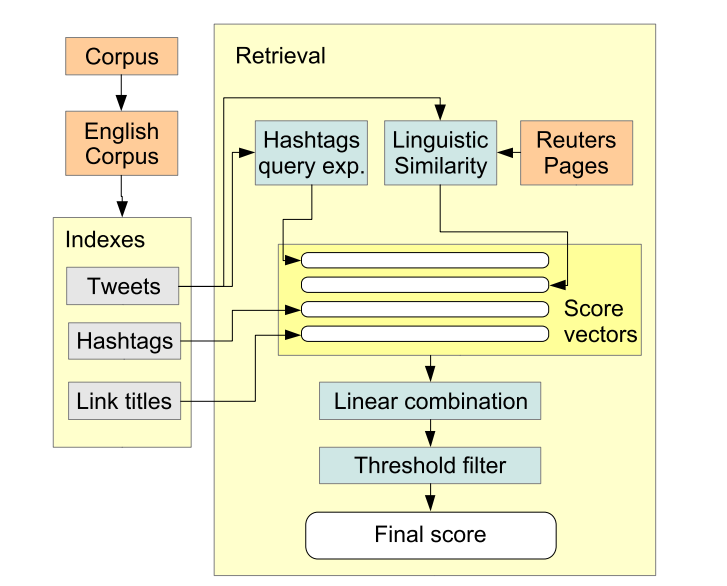
\includegraphics[width=5in]{paper1_2.png}
\caption{Modules of System}\label{fig:paper1}
\end{figure}

They used the words distribution model and a hashtag, the hashtag segmentation module converts the hashtag to a vector of words composing them. Finally, the last figure related to that paper is about how big dataset's size is.

\begin{figure}[htbp]
\centering
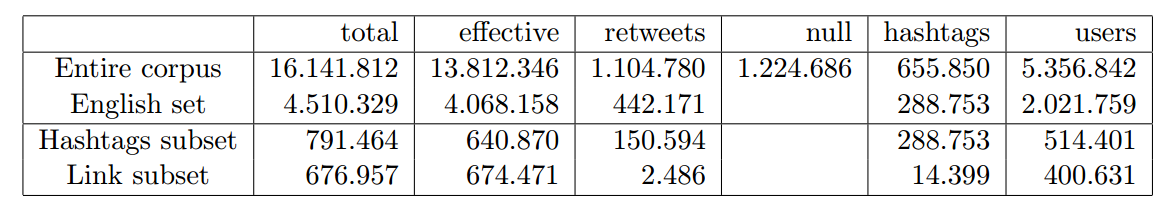
\includegraphics[width=7in]{paper1.png}
\caption{Some statistics from the corpus and the subsets that is selected for indexing,
the total number of tweets is divided in effective tweets, retweets and null tweets. 
The hashtags column indicates the number of unique hashtags.}\label{fig:paper1}
\end{figure}

\subsubsection{Segmenting Web-Domains and Hashtags using Length Specific Models}
In this project, they study two applications in the internet domain. First application
is the web domain segmentation which is crucial for monetization
of broken URLs. Secondly, they propose and study a novel application of twitter hashtag 
segmentation for increasing recall on twitter searches. They remark that existing methods for
word segmentation use unsupervised language models. 

They have realized that when using multiple corpora, the joint probability model from multiple corpora performs significantly better
than the individual corpora during the project. Motivated by this, they propose
weighted joint probability model, with weights specific
to each corpus. Finally, they observed that length of segments is an important parameter for word segmentation.
The length specific models further improve segmentation accuracy
over supervised probability models.

\subsubsection{A Simple and Effective Unsupervised Word Segmentation Approach}
In this paper, they propose a new unsupervised algorithm to achieve word segmentation. The main idea of their approach
is a novel word induction criterion which is similar with second paper. As they explain; ``We devise a method
to derive exterior word boundary information from the
link structures of adjacent word hypotheses and incorporate
interior word boundary information to complete
the model.''\footnote{A Simple and Effective Unsupervised Word Segmentation Approach, Songjian Chen, Yabo Xu, Huiyou Chang}
They have also worked with Chinese datasets to claim their approach. If it is working with even difficult language systems, it will be achieved with other systems. They also reported that their approach is simpler and more efficient than the Bayesian methods and more suitable for real-world applications.

\begin{figure}[htbp]
\centering
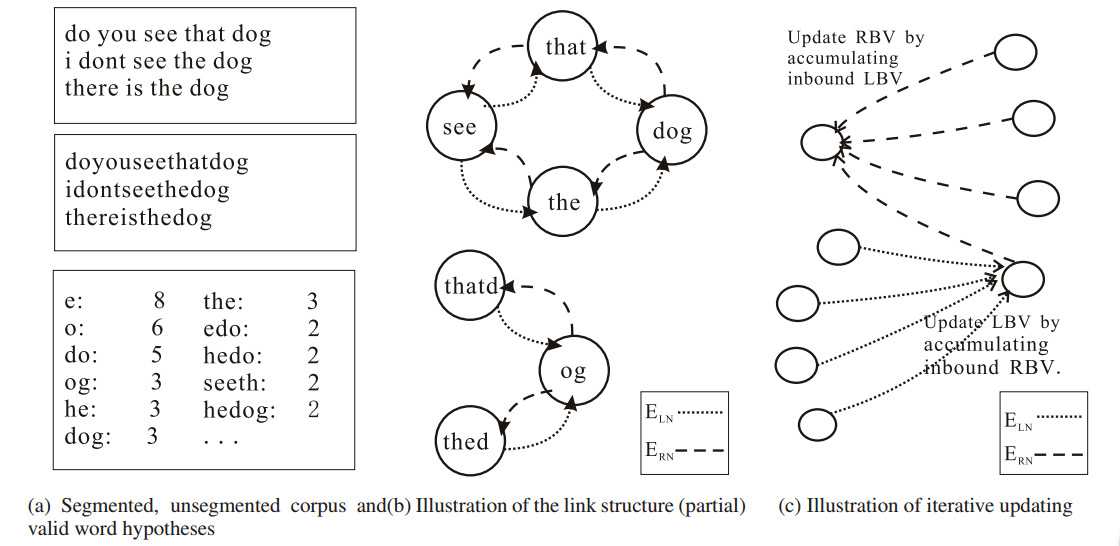
\includegraphics[width=7in]{paper3.png}
\caption{Illustrations of constructing the link structures of word hypotheses and calculating the exterior boundary values.}\label{fig:paper1}
\end{figure}

\subsubsection{URL Segmentation}
Another approach is word segmentation of URL links. To think about the word segmentation and
recognition problem for URL links, reasearchers adopt some basic principles from rule­based
approach.

The dictionary should have sufficient amount of word entries. However, the occurence
of compound words makes it very difficult to match every component string exactly with the
dictionary entries. Evaluation of the hashtag segmentation has started to be improved with search engine
improvements of Twitter.

Finite state transducer is an approach for title token base URL segmentation. It splits and segments according to previous-seen web page title simultaneously. For example, URL link includes "cs" that might correspond to "computer science" in many training page's title. If "cs" is encountered in the testing corpus, it is automatically expanded to "computer science". The tranducer has several rules that give score. This score can be obtain by certain moves which match or skip letters in the tokens of title with corresponding letters. Expansion can be valid if it covers all letters in the segment.


\subsection{Improvement of Our Project}
In our project, there are several improvements according to local and global researches. Firstly, as we mentioned before, it is the first project that introduces a platform for segmentation of Twitter hashtags in Turkish. We also gathered datasets from Twitter and parse them into "tweet body" and "hashtags". We have used maximum entropy model to separate words. We have also imlement an application feature to embed project into any platform. If we get hashtags, we can return the segmented version of them


\section{Methods}
\subsection{Current Methods}
We will discuss two types of models and both models focus on words, not boundaries. And they also use little or no domain-specific information.

\subsubsection{Parser Model}
No special mechanism is needed for word segmentation; it results from interaction of perception
and internal representation. Humans are not tracking boundary statistics; segmentation results from general properties of attention, perception, and memory.

Initially, input is perceived and chunked randomly into units;
\begin{itemize}
\item Units are encoded in memory.
\item Memory decays rapidly.
\item Uncommon units disappear, common units are reinforced.
\item Units in memory influence perception and encoding of new input (input is segmented into existing units).
\end{itemize}

\begin{figure}[htbp]
\centering
\includegraphics[width=2in]{parser.png}
\caption{Parser System}\label{fig:parser}
\end{figure}

The properties of parser model;
\begin{itemize}
\item No explicit tracking of statistics is needed.
\item Works on experimental stimuli but might need modifications for realistic language.
\item Probably would work in many domains.
\end{itemize}

\subsubsection{Bayesian Model}
Bayesian model has two varieties in the case of words, that is, whether they are independent from eachother or dependent on other words. If they are independent, we are talking about unigram models. However, if words are dependent on others from same corpus, we are talking about bigram models.

The working data is unsegmented corpus for bayesian models. This hypotheses works on sequences of word tokens.
It introduces optimal solution with highest prior probability.

The properties of bayesian model;
\begin{itemize}
\item Good segmentations of naturalistic data can be found using fairly weak/domain-general prior assumptions.
\item Utterances are composed of discrete words.
\item Units tend to be short.
\item Some units occur frequently, most do not.
\item Units tend to come in predictable patterns.
\item More sophisticated use of information works better.
\end{itemize}

\subsection{Our Method}
We used "git" as a version control system. Our version history is as follows.

\begin{center}
\begin{tabular}{ | l | p{10cm} |}
\hline
Date & Action\\ \hline
17 October, 2015 & Twitter API update is done.\\ \hline
8 November, 2015 & Datasets are created and parsing them into database is completed.\\ \hline
9 November, 2015 & First Report (Midterm Report) and database upgrades(tweet body and hashtags are seperated) are done.\\ \hline
14 November, 2015 & Midterm Report is finished.\\ \hline
15 December, 2015 & Hashtag verification is extended.\\ \hline
16 December, 2015 & Random hashtags are created for test data.\\ \hline
9 January, 2016 & Four features are implemented for learning data(Maximum Entropy Model).\\ \hline
10 January, 2016 & Maximum Entropy Model is created with current learning data.\\ \hline
12 January, 2016 & Final Project Report, video presentation, application and poster are added.\\ \hline
13 January, 2016 & Final delivery is done.\\
\hline
\end{tabular}
\end{center}

When we started working on the project, there were no datasets for machine learning algorithm and some testing features.
Very beginning of the project, we have decided to use "python" as main programming language, because we work on languages, that is, contains a lot of text data. It is knowns off as scripting language. There are several scripting languages as perl, ruby etc. But in the case of size of community and finding efficient APIs, python has more power on them.

\begin{figure}[htbp]
\centering
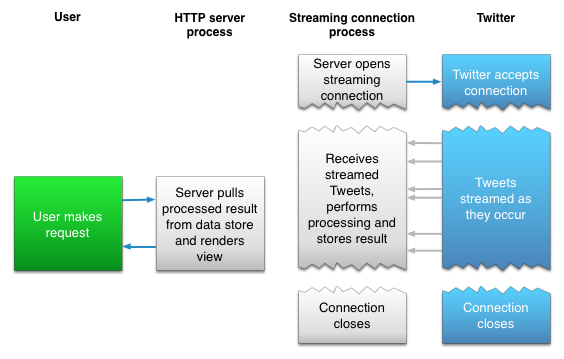
\includegraphics[width=4in]{streaming.png}
\caption{Twitter Streaming API}\label{fig:api}
\end{figure}

We started to gather data from "Twitter" via their developer accounts. We create a Twitter account and sign up for developer account. We get developer keys and embed them into streaming Twitter API which is "tweepy" After that, we began to collect tweets in ".json" format which includes lots of information about tweets. We decided to extract tweet bodies and ID's.

\begin{figure}[htbp]
\centering
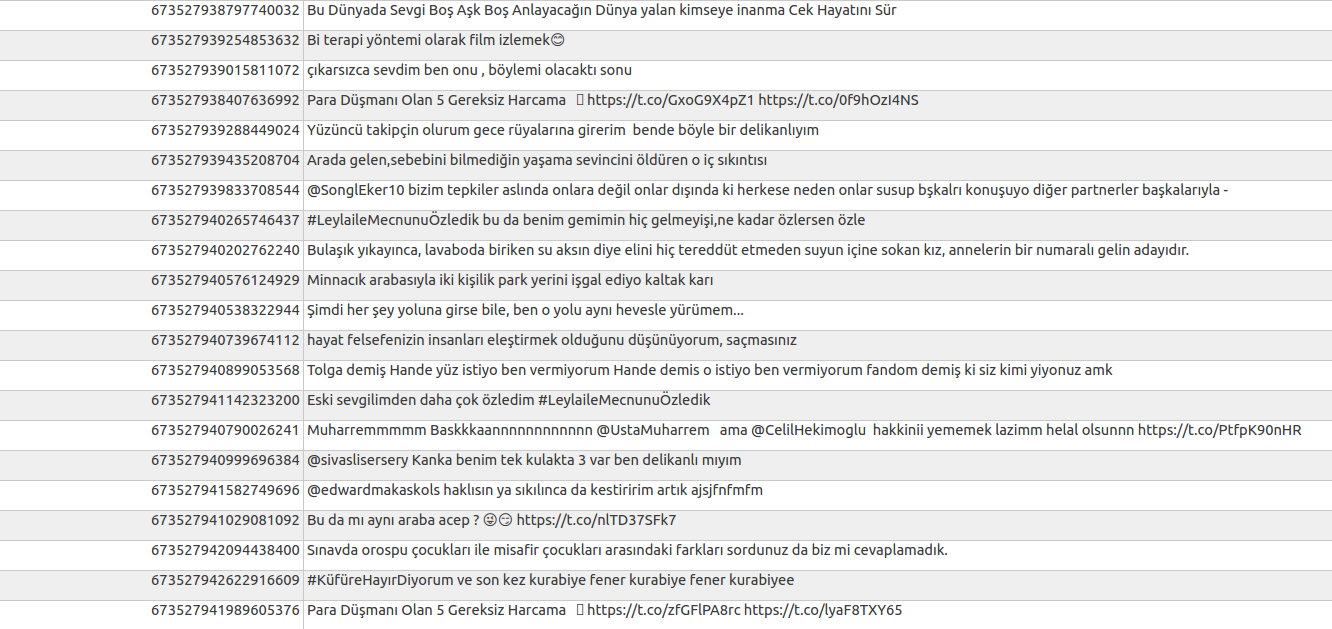
\includegraphics[width=7in]{textdatabase.png}
\caption{Tweet body examples from training corpus}\label{fig:model}
\end{figure}

\begin{figure}[htbp]
\centering
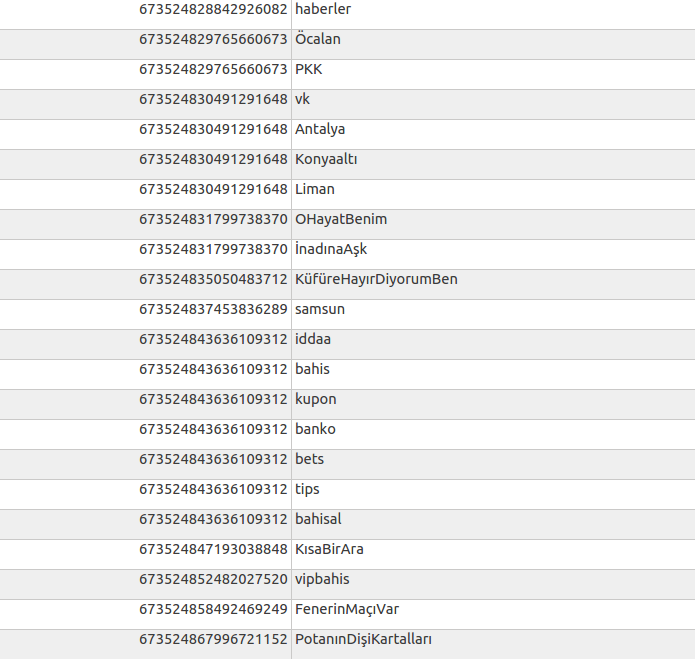
\includegraphics[width=4in]{hashtagdatabase.png}
\caption{Tweet hashtag examples from training corpus}\label{fig:api}
\end{figure}

After extracting action, we gathered hashtags from bodies in the way of hashtag rules. Meanwhile extracting hashtags from bodies, we stored them (body, ID, hashtags) into database. We used "sqlite" as database tool.

\begin{figure}[htbp]
\centering
\includegraphics[width=4in]{Model.png}
\caption{The Way of Implementation}\label{fig:model}
\end{figure}

In order to create learning data, we used tweet bodies from our corpus. URLs, hashtags and some parts as well as "@" symbols are removed. We put them together if there is a posibility to have a meaningful parts. In order to mark word boundaries we used "~" as our marker. This action helped us to create useful learning data.

After created learning data, we have decided to use four features for our model. Feature mechanism is unique for models. Features can be extended to improve our results. In addition to that, vocabulary of corpus may be used to get better results.

Features are determined in terms of ease of implementation. Getting convenient results can be only improved on working systems.

They are as follows;
\begin{itemize}
\item m1: It has current and next two characters as lower case. It includes "@" in the case of out of bounds.
\item m2: It has current and next two characters as no lower or uppercase action. It includes "@" in the case of out of bounds.
\item m3: It checks current and next two characters. It writes "x" for lowercase, "X" for uppercase and "@" for out of bounds situation.
\item m4: It checks previous, currend and next characters. It writes "x" for lowercase, "X" for uppercase and "@" for out of bounds situation.
\end{itemize}

\begin{figure}[htbp]
\centering
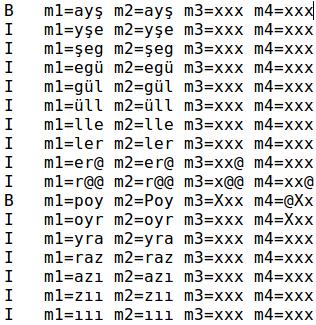
\includegraphics[width=3in]{train.png}
\caption{Our feature example from training corpus}\label{fig:model}
\end{figure}

In order to create test data, we get 1000 random hashtags from our database. We seperate words manually. Finally, we have one original test data and one manually seperated test data to calculate precision, recall, f-measure and accuracy.

\subsubsection{Maximum Entropy Model}

The target of statistical modeling is to contruct a model that fits best accounts for training data. More spesifically, for given training data, we have probability distrubution. We want to build a model that is close to training probability as possible.

\begin{figure}[htbp]
\centering
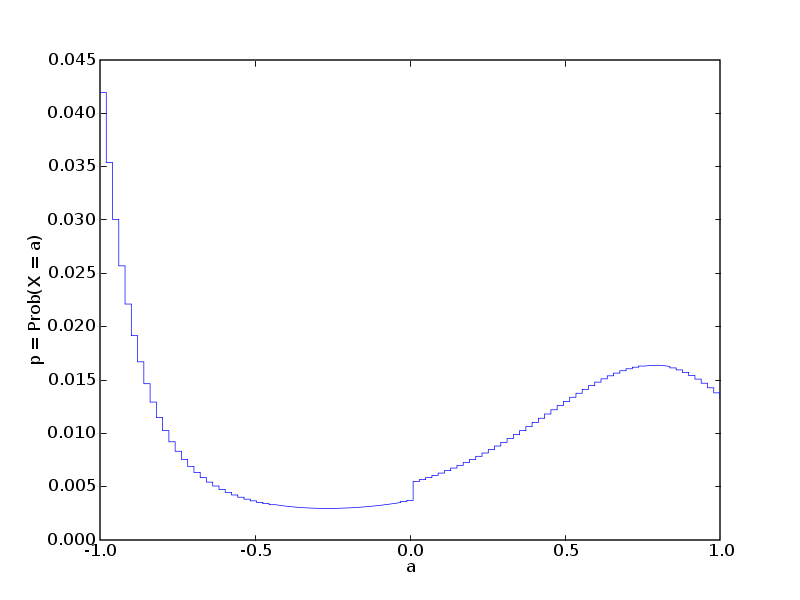
\includegraphics[width=4in]{mem.jpg}
\caption{Maximum Entropy Model Distribution}\label{fig:model}
\end{figure}

We have used "Maximum Entropy Model" to decide boundaries of words. The Maximum Entropy model can be introduced as; "The modeler can choose arbitrary feature functions in order to reflect the characteristic of the problem domain as faithfully as possible. The ability of freely incorporating various problem-specific knowledge in terms of feature functions gives ME models the obvious advantage over other learn paradigms, which often suffer from strong feature independence assumption (such as naive bayes classifier)."\footnote{Le, Zhang, Maximum Entropy Modeling Toolkit
for Python and C++, 29th December 2004}

We created Model with training data via maximum-entropy model. We create features for original test data. After that, we give that data to maximum-entropy tool and in terms of results from tool, hashtags are segmented. We added segmented hashtags which are calculated by tool and manually segmented hashtags to text file. It helps us to calculate precision, recall, f-measure and accuracy of segmentation method.

\begin{figure}[htbp]
\centering
\includegraphics[width=5in]{Exetool.png}
\caption{Methods of Segmentation}\label{fig:model}
\end{figure}

\section{Results}
In brief, we have collected the tweets from twitter. We tokenize tweets, normalize them and get 
hashtags from them. We have stored all information related to tweets. That will help us to recognize training and test data. The training and the test data were the part of the current data. We created model from learning data and boundaries of words are decided. At the end of the progression we calculated the measurements of result.

\begin{center}
\begin{tabular}{| l | l | p{10cm} |}
\hline
Precision & 75.51\\ \hline
Recall & 64.80\\ \hline
F-Measure & 69.75\\ \hline
Accuracy & 49.57\\ \hline
\# of Unique Tweets & 1.169.282\\ \hline
\# of Unique Hashtags & 24.003\\
\hline
\end{tabular}
\end{center}

\section{Discussion and Conclusion}
\subsection{Discussion}
There are several methods to achieve word segmentation. As we mentioned, Maximum Entropy Model is used. We may use different methods, but we decided max-ent that gives us best results.

\subsection{Conclusion}
We have researched our project and get respectable amount of results. Our results are good enough but it can always be improved by computer science developers. It is an open source project and we hope it will help researches in natural language processing field.

\section{Future Work}
Future works to increase segmentation results can be as follows;
\begin{itemize}
\item Vocabulary of corpus feature can be added.
\item More than four features can be added.
\item The size of corpus can be extended.
\item The irrelevant data can be removed from corpus.
\item The hashtags which contain foreign words can be removed.
\end{itemize}

\section{References}
- Berardi, Giacomo; Esuli, Andrea; Marcheggiani, Diego and Sebastiani, Fabrizio. Exploring the use of hashtag segmentation and text quality ranking 
Istituto di Scienza e Tecnologie dell’Informazione Consiglio Nazionale delle Ricerche 56124 Pisa, Italy

- Kan, Min-Yen, Web Page Classification

- Bansal, P., Bansal, R. and Varma V. 2015. Towards
Deep Semantic Analysis Of Hashtags.

- Berardi, G. and Esuli, A. and Marcheggiani, D. and
Sebastian, F. 2011. ISTI@TREC Microblog track
2011: exploring the use of hashtag segmentation
and text quality ranking.

- Chen, S. and Xu Y. and Chang, H. 2012. A Sim-
ple and Effective Unsupervised Word Segmentation
Approach. Proceedings of the Twenty-Fifth AAAI
Conference on Artificial Intelligence

- Xue, N. 2003. Chinese word segmentation as charac-
ter tagging.. International Journal of Computational
Linguistics and Chinese Language Processing vol-
ume 8(1)

- Wong, P and Chan, C. 1996. Chinese word segmenta-
tion based on maximum matching and word binding
force.
\nocite{*}

\bibliographystyle{compj}
\bibliography{ModellingBidders}

\section{Appendix}

\end{document}